%\RequirePackage[l2tabu, orthodox]{nag}
\documentclass[12pt]{beamer}
\newenvironment{ConCodigo}[1]
  {\begin{frame}[fragile,environment=ConCodigo]{#1}}
  {\end{frame}}
\graphicspath{{Imagenes/}{../Imagenes/}}
\usepackage[utf8]{inputenc}
\usepackage[spanish]{babel}
\usepackage{hyperref}
\usepackage{etex}
\reserveinserts{28}
\usepackage{amsmath}
\usepackage{amsthm}
\usepackage{mathtools}
\usepackage{multicol}
\usepackage{multirow}
\usepackage{tabulary}
%\usepackage{tabularx}
\usepackage{booktabs}
\usepackage{nccmath}
\usepackage{biblatex}
\usepackage{epstopdf}
\usepackage{graphicx}
\usepackage{siunitx}
\sisetup{scientific-notation=true}
%\usepackage{fontspec}
\usepackage{lmodern}
\usepackage{float}
\usepackage[format=hang, font=footnotesize, labelformat=parens]{caption}
\usepackage[autostyle,spanish=mexican]{csquotes}
\usepackage{standalone}
\usepackage{tikz}
\usepackage[siunitx]{circuitikz}
\usetikzlibrary{arrows,patterns,shapes}
\usetikzlibrary{decorations.markings}
\usetikzlibrary{arrows}
\usepackage{color}
%\usepackage{beton}
%\usepackage{euler}
%\usepackage[T1]{fontenc}
\usepackage[sfdefault]{roboto}  %% Option 'sfdefault' only if the base font of the document is to be sans serif
\usepackage[T1]{fontenc}
\renewcommand*\familydefault{\sfdefault}
\DeclareGraphicsExtensions{.pdf,.png,.jpg}
\usepackage{hyperref}
\renewcommand {\arraystretch}{1.5}
\newcommand{\python}{\texttt{python}}
\usefonttheme[onlymath]{serif}
\setbeamertemplate{navigation symbols}{}
\usetikzlibrary{patterns}
\usetikzlibrary{decorations.markings}
\tikzstyle{every picture}+=[remember picture,baseline]
%\tikzstyle{every node}+=[inner sep=0pt,anchor=base,
%minimum width=2.2cm,align=center,text depth=.15ex,outer sep=1.5pt]
%\tikzstyle{every path}+=[thick, rounded corners]
\setbeamertemplate{caption}[numbered]
\newcommand{\ptm}{\fontfamily{ptm}\selectfont}
%Se usa la plantilla Warsaw modificada con spruce
\mode<presentation>
{
  \usetheme{Warsaw}
  \setbeamertemplate{headline}{}
  \useoutertheme{default}
  \usecolortheme{beaver}
  \setbeamercovered{invisible}
}
\AtBeginSection[]
{
\begin{frame}<beamer>{Contenido}
\normalfont\mdseries
\tableofcontents[currentsection]
\end{frame}
}

\usepackage{media9}
\usepackage{siunitx}
\usepackage{standalone}
\usepackage{longtable}
\newcommand*{\TitleParbox}[1]{\parbox[c]{6cm}{\raggedright #1}}%
\usepackage{listings}
\lstset{ %
language=Python,                % choose the language of the code
basicstyle=\small,       % the size of the fonts that are used for the code
numbers=left,                   % where to put the line-numbers
numberstyle=\small,      % the size of the fonts that are used for the line-numbers
stepnumber=1,                   % the step between two line-numbers. If it is 1 each line will be numbered
numbersep=5pt,                  % how far the line-numbers are from the code
backgroundcolor=\color{white},  % choose the background color. You must add \usepackage{color}
showspaces=false,               % show spaces adding particular underscores
showstringspaces=false,         % underline spaces within strings
showtabs=false,                 % show tabs within strings adding particular underscores
frame=single,   		% adds a frame around the code
tabsize=2,  		% sets default tabsize to 2 spaces
captionpos=b,   		% sets the caption-position to bottom
breaklines=true,    	% sets automatic line breaking
breakatwhitespace=false,    % sets if automatic breaks should only happen at whitespace
escapeinside={\%},          % if you want to add a comment within your code
stringstyle =\color{magenta},
keywordstyle = \color{blue},
commentstyle = \color{green},
identifierstyle = \color{red}
}
\title{Tema 1 - Escalas, condición y estabilidad}
\subtitle{Curso de Física Computacional}
\author[]{M. en C. Gustavo Contreras Mayén}
\date{}
\begin{document}
\maketitle
\fontsize{14}{14}\selectfont
\spanishdecimal{.}
\section{Objetivo}
\begin{frame}
\frametitle{Objetivo}
Al concluir el Tema 1, el alumno:
\begin{enumerate}
\item En el diseño de algoritmos para la solución numérica de problemas de la física, aplicará los conceptos de: \textit{Condición}, \textit{Estabilidad} y \textit{Eficiencia}, apoyándose en la teoría de representación de números en la computadora y de la teoría de propagación de errores.
\end{enumerate}
\end{frame}
\section{Introducción a la Física Computacional}
\begin{frame}
\frametitle{¿Qué es la física computacional?}
La física computacional es una nueva manera de hacer investigación en física, próxima al
experimento y a la teoría.
\\
\medskip
En el laboratorio se realizan mediciones en sistemas físicos reales (restringida a la factibilidad de recursos técnicos), y que luego los físicos teóricos explican esas mediciones mediante las teorías.
\end{frame}
\begin{frame}
\frametitle{Areas de investigación en la física}
\begin{itemize}[<+->]
	\item Problemas que no tienen solución analítica.
	\item Validar aproximaciones y hacer efectivas las teorías propuestas.
	\item Comparar cuantitativamente teorías y mediciones experimentales.
	\item Visualizar conjuntos de datos complejos.
	\item Control y medición de experimentos.
\end{itemize}
\end{frame}
\begin{frame}
\fontsize{14}{14}\selectfont
\begin{multicols}{2}
\begin{itemize}[<+->]
	\item Predicción del clima
	\item Superconductividad
	\item Genoma Humano
	\item Visión y lenguaje
	\item Fusión nuclear
	\item Oceanografía
	\item Ciencia de los materiales
	\item Diseño de semiconductores
	\item Astrofísica relativista
	\item Sistemas de combustión
	\item Estructura biológica
	\item Diseño de fármacos
	\item Turbulencia
	\item Recuperación de petróleo y gas
	\item Cromodinámica cuántica
\end{itemize}
\end{multicols}
\end{frame}
\begin{frame}
\begin{center}
\begin{tikzpicture}[scale=0.8]
\begin{scope}[fill opacity=0.7]

\draw [fill=yellow, thin] (0,3.5) circle (2);\pause
\draw [font=\small] (0,3.5) node {Física};

\draw [fill=blue, thin] (-2.4,-2.4) circle (2);\pause
\draw [font=\small] (-2.4,-2.4) node {Ciencias};
\draw [font=\small] (-2.4,-2.9) node {de la Computación};

\draw [fill=orange, thin] (2.4,-2.4) circle (2);\pause
\draw [font=\small] (2.4,-2.4) node {Matemáticas};

\draw [fill=gray, thin] (0,0) circle (2.5);\pause
\draw [font=\small] (0,0) node {Física Computacional};
\end{scope}
\end{tikzpicture}
\end{center}
\end{frame}
\begin{frame}
\frametitle{Alcance del curso}
El curso está diseñado para ofrecer una introducción a los métodos numéricos aplicados a la física.
\\
\medskip
Se da un punto de referencia para continuar profundizando de manera particular en temas específicos. El desarrollo de las habilidades de programación, están en función del tiempo dedicado al trabajo fuera de la clase, pero consideramos que se abren un panorama diferente para abordar ya sea un servicio social, tesis o proyecto de trabajo para un posgrado.
\end{frame}
%\begin{frame}[fragile]
%\frametitle{Ejemplos avanzados de programación con \python}
%\begin{itemize}
%	\item Pelota rebotando. % \href{run:C:\\Python27\\Lib\\site-packages\\visual\\examples\\bounce.py}
%	\item Péndulo doble.
%	\item Conjunto de Mandelbrot.
%	\item Gas.
%	\item Estrellas
%\end{itemize}
%\end{frame}
%\begin{frame}
%\frametitle{Video}
%\includemedia[
%width=1.0\linewidth,height=0.667\linewidth, % 16:9activate=pageopen,
%flashvars={
%modestbranding=1 % no YT logo in control bar
%&autohide=1 % controlbar autohide
%&showinfo=0 % no title and other info before start
%&rel=0 % no related videos after end
%}]{}{https://www.youtube.com/v/EMVBLg2MrLs?rel=0}
%\end{frame}
\section{Conceptos principales}
\begin{frame}
\frametitle{Método numérico}
Se puede representar como una cadena de algoritmos $A_{i}$ con $(i = 1, 2, 3, \ldots , N)$ en la entrada y salida.
\begin{figure}
\centering
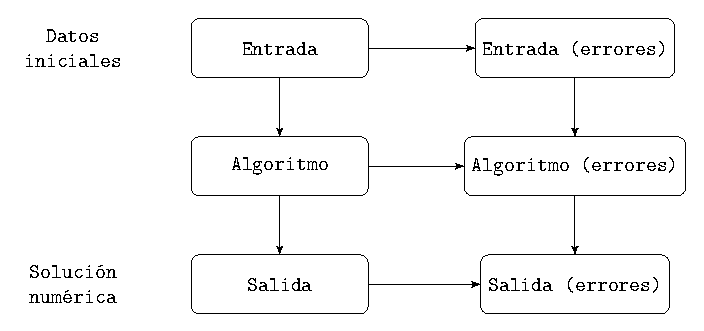
\includegraphics[scale=1]{dibujometodonum.eps} 
\end{figure}
\end{frame}
\begin{frame}
La solución obtenida por un método numérico es \textcolor{blue}{aproximada}, es decir, hay cierta diferencia entre la solución exacta y la solución numérica.
\end{frame}
\begin{frame}
\frametitle{Principales causas de la diferencia}
\begin{itemize}[<+->]
\item Falta de correspondencia entre el problema (modelo) matemático y el fenómeno físico real.
\item Errores en los datos iniciales (parámetros de entrada).
\item Errores en el método numérico usado para resolver el problema.
\item Errores de redondeo en las operaciones aritméticas.
\end{itemize}
\end{frame}
\section{Conceptos principales relacionados con modelos y métodos numéricos}
%\section{\texorpdfstring{this is a very long title I \\ want to}{want to break manually}}
\begin{frame}
\frametitle{Conceptos principales relacionados con modelos y métodos numéricos}
\begin{itemize}[<+->]
\item Aproximación.
\item Estabilidad.
\item Convergencia.
\end{itemize}
\end{frame}
\begin{frame}
\frametitle{Aproximación}
Es la proximidad de un modelo numérico al modelo original (diferencial, integral, etc.) o el
grado de aproximación, caracteriza el error que se introduce al hacer discreto el modelo
continuo.
\\
\bigskip
El grado de aproximación $n$ se estima mediante un factor que tiene el error entre dos modelos.
\end{frame}
\begin{frame}
\frametitle{Estabilidad}
\begin{itemize}[<+->]
\item Caracteriza la manera de propagación de los errores iniciales dentro del algoritmo en el
proceso del cálculo.
\item Si el incremento de errores iniciales es considerable y sin ningún control, entonces el
método numérico se llama \textcolor{red}{inestable}.
\item Si los errores de cálculos dependen continuamente de los errores iniciales, entonces el método se llama \textcolor{blue}{estable}.
\end{itemize}
\end{frame}
\begin{frame}
\frametitle{Convergencia}
\begin{itemize}
\item  Significa que la solución numérica converge hacia la solución exacta cuando el tamaño de la malla $h$ tiene a cero, o el número de truncación $N$ tiende al infinito.
\end{itemize}
\end{frame}
\section{Errores en los métodos numéricos}
\begin{frame}
\frametitle{Errores en los métodos numéricos}
\begin{itemize}[<+->]
\item \textcolor{brown}{Truncamiento}: se debe a las aproximaciones utilizadas en la fórmula
matemática del modelo.
\item \textcolor{orange}{Redondeo}: se asocia al hecho de que la representación de un número en la computadora se hace con un conjunto limitado de dígitos.
\end{itemize}
\end{frame}
\begin{frame}
\frametitle{Series de Taylor}
\begin{itemize}[<+->]
\item Las soluciones numéricas son en su mayoría, aproximaciones de las soluciones exactas.
\item Gran parte de los métodos numéricos se basan en la aproximación de funciones por medio de polinomios.
\end{itemize}
\end{frame}
\begin{frame}
El desarrollo de Taylor es una serie infinita de potencias, representa de manera exacta a una función dentro de un cierto radio alrededor de un punto dado.
\\
\medskip
Al comparar el desarrollo polinomial de la solución numérica con la serie de Taylor de la solución exacta, es posible evaluar el error, conocido como error de \textcolor{blue}{truncamiento}.
\end{frame}
\begin{frame}
Si se ignoran todos los términos de la serie de Taylor, excepto algunos cuantos, se puede obtener un polinomio que se aproxime a la función verdadera.
\\
\medskip
A éste polinomio se le llama \textit{serie de Taylor truncada} y se usa como punto de partida para obtener métodos numéricos.
\end{frame}
\begin{frame}
\frametitle{Definición de Serie de Taylor}
Una función $f(x)$ es analítica en $x=a$ si $f(x)$ se puede representar por medio de una serie de potencias en términos de $h = x-a$ dentro de un radio de convergencia $D > |x-a|> 0$.
\\
\bigskip
Una condición necesaria para que una función sea analítica es que todas sus derivadas sean continuas tanto en $x=a$ como en alguna vecindad alrededor de ese punto.
\end{frame}
\begin{frame}
Un punto en donde una función $f(x)$ no es analítica recibe el nombre de punto singular. 
\\
\medskip
Si $f(x)$ es diferenciable en todas las partes de la vecindad de $x_{0}$, excepto en $x_{0}$ , entonces $x_{0}$ es un punto singular.
\\
\medskip
Los polinomios son analíticos en todas partes.
\end{frame}
\begin{frame}
Si $f$ es analítica alrededor de $x = a$, se puede representar $f(x$) de manera exacta en la
vecindad de $x = a$ por medio de una serie de Taylor, dada por:
\fontsize{14}{14}\selectfont
\[ \begin{split} 
f(x) = f(a) + hf'(a) + \dfrac{h^{2}}{2} f''(a) + \dfrac{h^{3}}{6} f'''(a) + \ldots \\
+ \ldots + \dfrac{h^{m}}{m!} f^{m}(a) + \ldots
\end{split}
\]
\end{frame}
\begin{frame}
La serie de Taylor es única, esto quiere decir que no existe otra serie de potencias en $h = x-a$ para representar $f(x)$
\\
\bigskip
El desarrollo de Taylor de una función alrededor de $x = 0$ recibe el nombre de serie de Maclaurin.
\end{frame}
\begin{frame}
En aplicaciones prácticas, se debe de truncar la serie de Taylor después cierto orden, ya que es imposible incluir un número infinito de términos. Si la serie se trunca después del término $N$, se expresa por:
\[ \begin{split} f(x) &= f(a) + hf'(a) + \dfrac{h^{2}}{2} f''(a) + \dfrac{h^{3}}{6} f'''(a) + \ldots \\
&= + \ldots + \dfrac{h^{N}}{N!} f^{N}(a) + O(h^{N+1}) 
\end{split} \]
Donde $h=x-a$ y $O(h^{N+1})$ representa el error por el truncamiento de los términos de orden $N+1$
\end{frame}
\begin{frame}
El error global se puede representar como:
\[O(h^{N+1}) = f^{N+1}(a + \xi h) \dfrac{h^{N+1}}{(N+1)!} \hspace{1cm} 0 \leq \xi \leq 1\]
Dado que $\xi$ no puede calcularse con exactitud, se aproxima el término del error, haciendo $\xi = 0$
\[ O(h^{N+1}) \simeq f^{N+1}(a) \dfrac{h^{N+1}}{(N+1)!}\]
\end{frame}
\begin{frame}
Si $N=1$ la serie de Taylor truncada es:
\[f(x) \simeq f(a) + f'(a) h \hspace{1cm} h=x-a\]
incluyendo el efecto del error, tenemos que
\[f(x) \simeq f(a) + f'(a) h + O(h^{2}) \]
donde
\[O(h^{2}) \simeq f''(a+ \xi h) \dfrac{h^{2}}{2} \hspace{1cm} 0 \leq \xi \leq 1\]
\end{frame}
\begin{frame}
\frametitle{Redondeo con \python.}
\renewcommand*{\arraystretch}{2.5}
\begin{center}
%\captionof{table}{Funciones matemáticas intrínsecas}.
\begin{longtable}{| l | l |}
\hline
Función & Resultado \\ \hline
\endhead
\texttt{ceil (x)} & \TitleParbox{Redondea al valor entero mayor más cercano a $x$.} \\ \hline
\texttt{floor (x)} & \TitleParbox{Redondea al valor entero menor más cercano a $x$.} \\ \hline
\texttt{round (x [, n])} &  \TitleParbox{Devuelve el valor de $x$ redondeado a $n$ dígitos desde el punto decimal.} \\ \hline
\end{longtable}
\end{center}
\end{frame}
\begin{frame}[fragile]
\frametitle{Ejemplo con el código}
\begin{lstlisting}[columns=fullflexible]
from math import ceil, floor, pi

a = 10.4563

print('El valor de ceil(', a ,') es: ', ceil(a))

print('El valor de floor(', a ,') es: ', floor(a))

print('El valor de round(', a ,') es: ', round(a,3))

print('El valor de round(', pi ,',3) es: ', round(pi,3))
\end{lstlisting}
\end{frame}
\section{Representación de los números en las computadoras}
\begin{frame}
\frametitle{Base decimal}
El valor decimal de un número de base $r$ es
\[(abcdefg.hijk)_{r}\]
que se calcula como:
\begin{eqnarray*}
ar^{6} + br^{5} + cr^{4} + dr^{3} + er^{2} + fr +
 g + {} \\
{} + hr^{-1} + ir^{-2} + jr^{-3} + kr^{-4}
\end{eqnarray*}
\end{frame}
\begin{frame}
La menor y mayor magnitud de un número real que se pueden representar en una computadora, varían de acuerdo con el diseño tanto de hardware como de software.
\\
\bigskip
Los números reales en una computadora no son continuos. Si nos fijamos en número cercano a cero, el número positivo más pequeño en una IBM es $2.9 \times 10^{-39}$
\end{frame}
\begin{frame}
Por tanto, no se pueden representar números entre $0$ y $2.9 \times 10^{-39}$ 
\\
\bigskip
A éste intervalo se le conoce como \textcolor{blue}{épsilon de la máquina}.
\end{frame}
\begin{frame}
\frametitle{Epsilon de la máquina}
Hay dos maneras de definir el épsilon de la máquina: \textcolor{red}{un épsilon absoluto} y un \textcolor{blue}{épsilon relativo}.
\\
\bigskip
Este último es el más usado. Como el conjunto de números en la computadora es finito, la siguiente definición de épsilon relativo tiene sentido:
\[ \epsilon_{maq} = \epsilon = \min[t>0 : 1+t>1 ] \]
\end{frame}
\begin{frame}
El épsilon absoluto se define comparando con cero:
\[ \epsilon_{abs} = \min[t>0 : t \neq 0] \]
En realidad el épsilon depende de la máquina pero también del sistema operativo, del compilador y del tipo de números utilizados.
\end{frame}
\begin{frame}
\frametitle{Distribución de números reales en un computadora IBM PC}
\fontsize{10}{10}\selectfont
\begin{figure}
\centering
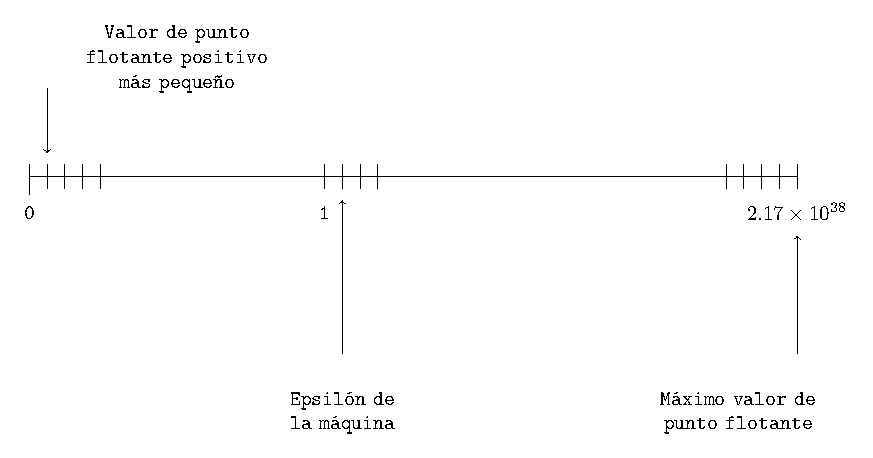
\includegraphics[scale=0.8]{epsilonmaquina.eps}
\end{figure}
\end{frame}
\begin{frame}[fragile]
\frametitle{Calculemos el epsilón con \python}
\begin{lstlisting}[columns=fullflexible]
t = 1.0;
while 1+t != 1:
  eps = t
  t = t/2
print ('el epsilon de la maquina es: ', eps)
\end{lstlisting}
\begin{figure}
\centering
\includegraphics[scale=1]{epsilonmaquina_02.eps}
\end{figure}
\end{frame}
\begin{frame}
\frametitle{Error de truncamiento}
Se originan al emplear al número finito de términos para calcular un valor que requiere un número infinito de términos.
\\
\bigskip
Por ejemplo, una expresión que permite determinar de forma exacta el valor del número de Euler (base de los logaritmos naturales) a través de una serie de MacLaurin es:
\[ e^{x} = \sum \dfrac{x_{i}}{i!}\]
\end{frame}
\begin{frame}
Sin embargo, una aproximación a dicho valor, puede obtenerse a través de su expresión finita:
\[ e^{x} \simeq \sum_{i=0}^{k} \dfrac{x_{i}}{i!} \hspace{1cm} k<\infty \]
Es claro que esta expresión finita es manejable computacionalmente hablando, al contrario que la fórmula expresada en su forma infinita.
\end{frame}
\begin{frame}
\frametitle{Error por redondeo}
Se origina por el hecho de que una computadora sólo puede representar un número finito de
términos. Para expresar una cantidad con un desarrollo decimal infinito, se tiene que prescindir de la mayoría de ellos.
\\
\bigskip
Por ejemplo, el número $\pi = 3.14159265 \ldots$, tiene un desarrollo decimal infinito no periódico. Por lo tanto, para fines de cálculo, sólo se toman algunos de sus dígitos.
\end{frame}
\begin{frame}
\frametitle{Estrategias}
\begin{itemize}[<+->]
\item \textcolor{blue}{Redondeo}. Prescinde de cierto número de cifras significativas y realiza un ajuste, sobre la última cifra no descartada: $\pi = 3.1416$
\item \textcolor{red}{Corte o poda}: Prescinde de cierto número de cifras significativas sin realizar un ajuste sobre la última cifra no descartada: $\pi = 3.1415$
\end{itemize}
\end{frame}
\section{Tipos de errores}
\begin{frame}
\frametitle{Nuevos conceptos}
Una vez que se ha establecido la clasificación del error, definiremos los conceptos de:
\begin{itemize}
\item \textcolor{red}{Error absoluto verdadero}.
\item \textcolor{orange}{Error relativo verdadero}.
\item \textcolor{blue}{Error relativo aproximado}.
\end{itemize}
todos ellos como una suma o consecuencia de los errores de redondeo y truncamiento.
\end{frame}
\subsection{Error absoluto verdadero}
\begin{frame}
\frametitle{Error absoluto verdadero}
Supóngase que $\widehat{p}$ es una aproximación a p.
\\
\bigskip
El error absoluto verdadero se define con la siguiente expresión:
\[ E_{v} = \vert p - \widehat{p} \vert \]
Esta definición de error, lo cuantifica en términos brutos. No obstante, una medida que puede describir con mayor detalle o proporción el error, es aquella que lo expresa en términos porcentuales. Para ello se emplea el error verdadero relativo.
\end{frame}
\subsection{Error relativo verdadero}
\begin{frame}
\frametitle{Error relativo verdadero}
Supóngase que $\widehat{p}$ es una aproximación a p. El error relativo verdadero se calcula con la siguiente expresión:
\[ e_{v} = \dfrac{\vert p - \widehat{p} \vert }{p}\]
El resultado suele expresarse en términos porcentuales.
\end{frame}
\subsection{Error relativo aproximado}
\begin{frame}
\frametitle{Error relativo aproximado}
El error relativo aproximado, mide el error de un método numérico, determinando el error de la iteración actual respecto el error surgido en la iteración anterior:
\[ e_{a} = \dfrac{\vert \widehat{x}_{i} - \widehat{x}_{i-1} \vert}{\widehat{x}_{i}}\]
Donde $x_{i}$ es la aproximación actual a $x$ y 
$x_{i-1}$ es la aproximación anterior a $x$.
\end{frame}
\begin{frame}
En métodos numéricos suele establecerse una tolerancia porcentual como criterio de paro, tal
que el error relativo aproximado de un método, no exceda dicha tolerancia.
\[ e_{a} < t \]
donde $t$, es tolerancia fijada de antemano. A menor tolerancia se tiene mayor precisión en la
aproximación al valor verdadero, sin embargo esto implica un aumento en el número de iteraciones requeridas para detener el método.
\end{frame}
\section{Contaminación en los cálculos}
\begin{frame}
\frametitle{Contaminación en los cálculos.}
Un error en un cálculo numérico ''contamina"" las sucesivas evaluaciones.
\\
\bigskip
Esta propagación puede describirse en términos de dos conceptos relacionados: los de estabilidad y condición.
\end{frame}
\subsection{Condición}
\begin{frame}
\frametitle{Condición}
La condición de una función $f(x)$ mide la sensibilidad de los valores de $f(x)$ a pequeños
cambios de $x$, se define como:
\[ C = \left | \dfrac{E_{rel} (f(x))}{E_{rel}(x)} \right |  \]
\end{frame}
\begin{frame}
Del teorema del valor medio en cálculo, podemos expresar
\[ \begin{split} f(x_{T}) - f(x_{A}) & \approx f'(x_{t})(x_{T} - x_{A}) \rightarrow E_{rel}(f(x)) \approx \\ 
 & \approx \dfrac{f'(x_{T})}{f(x_{T})} (x_{T} - x_{A}) \end{split} \]
luego
\[ C \approx \left | x_{T} \dfrac{f'(x_{T})}{f(x_{T})} \right | \]
\end{frame}
\begin{frame}
Se utilizará ésta definición como definición de condición para funciones $f(x)$ de una variable real.
\\
\bigskip
Entonces los números de condición serán
\[ C = \left | x \dfrac{f'(x)}{f(x)} \right | \]
\begin{enumerate}[<+->]
\item Para un $x$ dado $0 < C(x) < 1$ se dirá que el problema está bien condicionado, y cuanto menor sea $C$, mejor condicionado.
\item Si $C(x) > 1$, el problema estará mal condicionado.
\item Si $C(x) = 1$, el error relativo se mantiene.
\end{enumerate}
\end{frame}
\begin{frame}
\frametitle{Ejemplos}
 Las siguientes funciones están bien condicionadas?
\begin{enumerate}
\item $f(x) = \sqrt{x} \hspace{1.5cm} C(x) = ?$
\item $g(x) = x^{2}-1 \hspace{1.5cm} C(x) = ?$
\end{enumerate}
\end{frame}
\subsection{Estabilidad}
\begin{frame}
\frametitle{Estabilidad}
La estabilidad de un algoritmo describe la sensibilidad de un método numérico específico
respecto a los inevitables errores de redondeo cometidos durante su ejecución en aritmética de precisión finita.
\end{frame}
\begin{frame}
Consideremos la siguiente función:
\[ f(x) = \sqrt{x+1} - \sqrt{x} \]
Su número de condición es:
\[ C(x) = \left | x \dfrac{f'(x)}{f(x)} \right | = \dfrac{x}{2 \sqrt{x} \sqrt{x+1}}\]
Vemos que $C(x)< \frac{1}{2}$ para $x>0$, por lo que la función está bien condicionada pero ...
\end{frame}
\begin{frame}
El algoritmo para calcular $x$ de tal forma que se vayan realizando las operaciones, es:
\begin{enumerate}[<+->]
\item obtener $x$
\item $y = x + 1$
\item $f = sqrt(y)$
\item $g = sqrt(x)$
\item $h = f – g$
\end{enumerate}
\pause
es inestable para $x$ grandes, dado el paso 5, por lo que debemos de re-estructurar la función.
\end{frame}
\subsection{Eficiencia}
\begin{frame}
\frametitle{Eficiencia}
\emph{Debemos evitar que todo algoritmo sea inestable}. Si existieran varios métodos para evaluar una misma función, entonces conviene utilizar aquel que sea más eficiente, es decir, más rápido.
\\
\bigskip
\pause
\textcolor{blue}{Hay que aprovechar al máximo los recursos: hardware, software, algoritmos, para resolver problemas más complejos y no para resolver peor problemas simples.}
\end{frame}
\begin{frame}
Por ejemplo, para calcular $x**4$ para un $x$ dado, no es buena idea calcular $x**4.0$ (exponente en punto flotante).
\\
\bigskip
La mejor idea consiste en economizar el cálculo en dos pasos:
\begin{eqnarray*}
x2 &=& x*x \\
x4 &=& x2*x2
\end{eqnarray*}
y no un producto $x4=x*x*x*x$
\end{frame}
\begin{frame}
\frametitle{Ejemplo: Evaluación de polinomios}
Supongamos que queremos evaluar el polinomio:
\[ P(x) = 2 + 4x - 5 x^{2} + 2 x^{3} - 6 x^{4} + 8 x^{5} + 10 x^{6}\]
Contando con que cada potencia de exponente $k$ entero como $k-1$ productos, tendríamos que el total de productos para evaluar en forma directa es:
\[ 1+2+3+4+5+6=21\]
Además de seis sumas.
\end{frame}
\begin{frame}
Una mejora en el algoritmo , es calcular primero las potencias de forma sucesiva:
\begin{eqnarray*}
x^{2} & = & x*x \\
x^{3} & = & x*x^{2} \\
x^{4} & = & x*x^{3} \\
x^{5} & = & x*x^{4} \\
x^{6} & = & x*x^{5}
\end{eqnarray*}
De tal forma que se añade un producto por cada potencia, para un total de productos:
\[1+2+2+2+2+2=11\]
\end{frame}
\begin{frame}
Con el polinomio
\[ P(x)=2 + 4 x - 5 x^{2} + 2 x^{3} - 6 x^{4} + 8 x^{5} + 10 x^{6}\]
podemos mejorar el algoritmo de la siguiente manera
\fontsize{12}{12}\selectfont
\[ P(x) = 2 + x \left\lbrace 4 + x \left( -5 + x \left[ 2 + x \left(-6 +x \left\lbrace 8+x*10 \right\rbrace \right) \right] \right) \right\rbrace  \]
\end{frame}
\begin{frame}
Para evaluar un polinomio de grado $n$ en el que ninguno de los coeficientes es cero, se necesitan
\\
\medskip
\pause
\begin{tabular}{l l}
$\dfrac{n(n+1)}{2}$ & Productos para el primer método \\
$2n-1$ & para el segundo métodos \\
$n$ & para el tercero
\end{tabular}
\\
\medskip
Antes de escribir una línea de código, hay que revisar la manera en que podemos optimizar la solución del problema.
\end{frame}
\section{Algoritmo de Horner}
\begin{frame}
\frametitle{Algoritmo de Horner}
Dado el polinomio
\[ P(x) = a_{0} + a_{1} x + \ldots + a_{n} x^{n} \hspace{1cm} a_{n} \neq 0 \]
La evaluación de $P(x)$ para cierto valor de $x=z$ se puede realizar en $n$ pasos mediante:
\begin{eqnarray*}
b_{n} &=& a_{n} \\
b_{n-1} &=& a_{n-1} + z*b_{n} \\
b_{n-2} &=& a_{n-2} + z*b_{n-1} \\
\vdots \\
b_{0} &=& a_{0}+z*b_{1}
\end{eqnarray*}
\end{frame}
\begin{frame}
\frametitle{Pseudocódigo}
\begin{enumerate}[<+->]
\item $b_{n} = a_{n}$
\item repetir mientras $n>0$
\item $n = n-1$
\item $b=a_{n}+z*b$
\item volver al paso 2
\item $p(z)=b$
\end{enumerate}
\end{frame}
\begin{frame}
\frametitle{Completa la siguiente tabla}
\[ P(x)=2 + 4 x - 5 x^{2} + 2 x^{3} - 6 x^{4} + 8 x^{5} + 10 x^{6}\]
Evalúa el polinomio $P(x)$ en:
\\
\medskip
\begin{center}
\begin{tabular}{S | c}
$x$ & $P(x)$ \\
\hline -1.5 & \\
\hline -0.65 & \\
\hline 0.1 & \\
\hline 1.4 & \\
\hline 2.87 & 
\end{tabular}
\end{center}
\end{frame}
\begin{frame}
\frametitle{Resultado}
\[ P(x)=2 + 4 x - 5 x^{2} + 2 x^{3} - 6 x^{4} + 8 x^{5} + 10 x^{6}\]
El polinomio $P(x)$ evaluado es:
\\
\medskip
\begin{center}
\begin{tabular}{S[table-format=1.2] | S[table-format=4.5] }
%x & P(x) \\
\hline -1.5 & 0.78125 \\
\hline -0.65 & -4.50683 \\
\hline 0.1 & 2.35149 \\
\hline 1.4 & 98.55968 \\
\hline 2.87 & 6758.70245
\end{tabular}
\end{center}
\end{frame}
\begin{frame}
\frametitle{Extendiendo la respuesta al problema}
¿Cómo resolver el problema usando una función? ¿mostrando una tabla con formato de salida? usando una gráfica que muestre $P(x)$ y un conjunto de datos evaluados? ¿Evaluar el error relativo?
\\
\bigskip
Ya contamos con las herramientas necesarias para extender la respuesta al problema, en nuestro código podemos agregar funciones, ajustar formatos de salida en los resultados, graficar el polinomio y los puntos (o un conjunto diferente de puntos), y obtener el error relativo. Basta con que le dediquemos un poco más de tiempo.
\end{frame}
\begin{frame}
\frametitle{Pasos a resolver}
\begin{enumerate}
\item Conviene definir una función que resuelva la evaluación del método de Horner.
\item Para obtener el error relativo, se debe de evaluar el polinomio y considerar que los valores obtenidos, son los valores exactos.
\item Comparamos los resultados mediante una gráfica que represente los dos resultados de la evaluación.
\end{enumerate}
\end{frame}
\begin{frame}[fragile]
\frametitle{Resultado gráfico más completo}
En la gráfica se muestra un conjunto de datos que se evalúan y posteriormente con la función (en línea continua) se compara, podemos ver que los resultados son prácticamente los mismo.
\begin{figure}
	\centering
	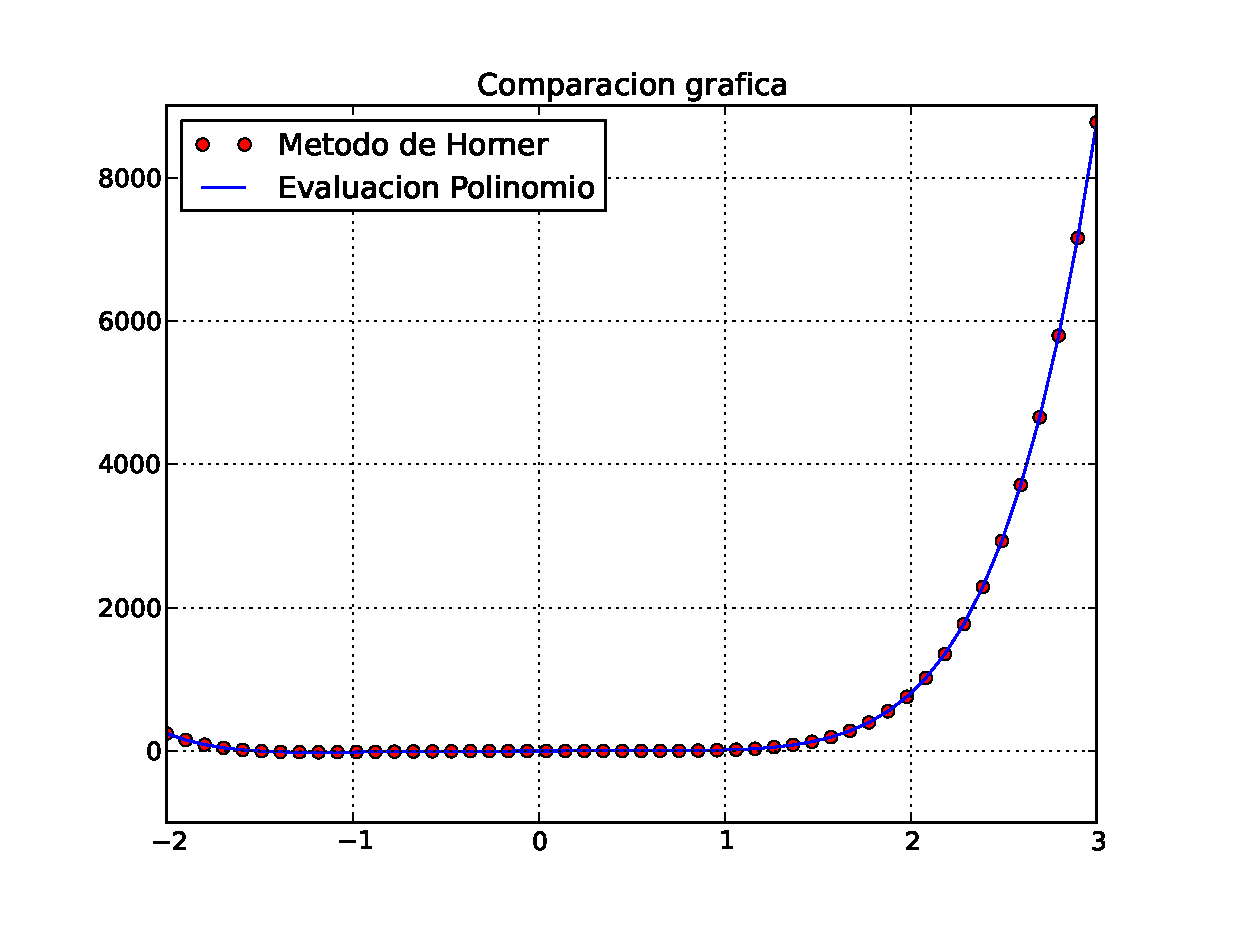
\includegraphics[scale=0.35]{MetodoHorner.eps} 
\end{figure}
\end{frame}
\begin{frame}[fragile]
\frametitle{Estructuramos el código en \python.}
Definimos mediante dos listas: 
\begin{enumerate}
\item Los valores donde queremos evaluar el polinomio $P(x)$.
\item Los coeficientes de $P(x)$.
\end{enumerate}
\begin{lstlisting}[basicstyle=\ttfamily\large, columns=fullflexible]
# Valores de x0 para evaluar P(x0)
x0=[-1.5, -0.65, 0.1, 1.4, 2.87]

# Coeficientes a de P(x)
a=[2,4,-5,2,-6,8,10]
\end{lstlisting}
\end{frame}
\begin{frame}[fragile]
\frametitle{Definimos una función que resuelva por Horner.}
\fontsize{14}{14}\selectfont
\begin{lstlisting}[basicstyle=\ttfamily\large, columns=fullflexible]
# Metodo de Horner

def P_Horner(x):
    P_Hor=0
    for n in range(len(a)-1,-1,-1):     
        P_Hor=a[n]+P_Hor*x
    return P_Hor
\end{lstlisting}
\end{frame}
\begin{frame}[fragile]
\frametitle{Definimos una función que evalúe directamente $P(x)$.}
\fontsize{14}{14}\selectfont
\begin{lstlisting}[basicstyle=\ttfamily\large, columns=fullflexible]
# Evaluacion directa

def P_Directo(x):
    return 2+4*x-5*x**2+2*x**3-6*x**4+8*x**5+10*x**6
    
\end{lstlisting}
\end{frame}
\begin{frame}[fragile]
\frametitle{Calculamos el error relativo.}
\fontsize{14}{14}\selectfont
\begin{lstlisting}[basicstyle=\ttfamily\large, columns=fullflexible]
# Calculo de error relativo

def Err_Rel(p,p_): return (p-p_)/p*100
    
\end{lstlisting}
\end{frame}
\begin{frame}[fragile]
\frametitle{Mostramos el error relativo de los puntos a evaluar.}
\fontsize{14}{14}\selectfont
\begin{lstlisting}[basicstyle=\ttfamily\large, columns=fullflexible]
# Evaluacion de valores de P(x0)

for i in range(len(x0)):                 
    print ("P(%.2f) =" %x0[i],P_Horner(x0[i]), "; Error rel. =", Err_Rel(P_Directo(x0[i]),P_Horner(x0[i])))
\end{lstlisting}
\end{frame}
\begin{frame}[fragile]
\frametitle{Comparamos los resultados con una gráfica.}
\fontsize{14}{14}\selectfont
\begin{lstlisting}[basicstyle=\ttfamily\small, columns=fullflexible]
import matplotlib.pyplot as plt
import numpy as np

x=np.linspace(-2.,3.)

plt.plot(x,P_Horner(x),'ro', label='Metodo de Horner')

plt.plot(x,P_Directo(x), label='Evaluacion Polinomio')

plt.title('Comparacion grafica')
plt.legend(loc='upper left')

plt.grid(True)
plt.show()
\end{lstlisting}
\end{frame}

\end{document}
